\chapter{What is an autonomous vehicle} \label{chap:two}
Before diving into the technical details that surround this project, it is crucial to make it clear what AV stands for and how the ideas of its development matured over the course of human history (\autoref{sect-2.1}). This chapter aims to give an overview of what makes an AV autonomous (\autoref{sect-2.2}), talks about the standardised way of classifying the autonomy levels in \autoref{sect-2.3} and discusses the AV safety vulnerabilities in \autoref{sect-2.4}.

\section{History of self-driving cars} \label{sect-2.1}
The idea of a self-driving car surprisingly reaches back as far as the 1500s when Leonardo Da Vinci designed his self-propelled cart \cite{fuller2008did} that could move without being pushed or pulled. Some regard this as the grandfather of today's automated vehicles. Although it might not have looked like something revolutionary, it shows that people living more than 400 years before the emergence of the first computer were already looking for ways to reduce human interaction in such basic everyday activities as pushing a cart.

In 1925, American engineer Francis Houdini tested the first driverless car that was operated using a remote-control setup that guided the car using radio signals \cite{engelking2017driverless}. Despite the fact that the car riding Manhattan streets demonstrated what an autonomous vehicle could look like, it did bring little success to the constructor. The project was shut down when the operator lost control of the vehicle twice and eventually crashed it into another vehicle.

Although the two occasions mentioned above sound like attempts to produce an autonomous vehicle, both Da Vinci's and Houdini's creations needed human input in their movement, whether winding the clog to start it or using the remote control device to decide its movements.

However, things changed forever when in 1958, almost twenty years after the initial concept was created, General Motors launched their prototype of a car that could ride the road on itself following a wire embedded into the asphalt. The concept was simple. The car contained sensors that could sense the current flowing through the wire, thus making it go according to the location of the wire and where it leads. It showed that a truly autonomous car has to be able to decide what to do by itself, relying on the data captured from the surrounding world.

This idea was reflected in the upcoming tries to create a self-driving vehicle. One includes a Japanese car built in 1977 that could slowly drive on the streets following the white street markers, and it could do so using cameras that were able to identify lane markings.
In 1995, researchers at Carnegie Mellon University developed a car called NavLab5 \cite{528266} that could steer itself on roads and highways using computers and video sensors. It was taken on an almost 3000 miles tour through the U.S., where it manoeuvred itself 98\% of the time, with human supervisors only needing to brake and throttle.

As highlighted by the organisation TWI Global - ``Today, a fully autonomous vehicle, is considered one that can operate itself and perform necessary functions without any human intervention through the ability to sense its surroundings.'' \cite{twi} 

One question that might arise is how exactly the vehicle would be able to know all its surroundings, determine what actions are legal and allowed, and navigate from one location to another without violating rules and causing harm to people or damaging properties. It might be about time to discuss the inside of an autonomous vehicle.

\section{What makes an AV} \label{sect-2.2}
At the core of an AV is a car with all the necessary parts for riding on the road. What distinguishes it from the cars that people are used to seeing is that it is equipped with multiple sensors providing all the necessary information about the world surrounding the vehicle. That data is then processed by the software responsible for all the logic and calculations that determine what commands need to be given to the semiconductors that make real-time driving actions.

Without sensors, the idea of an autonomous car would be impossible. They allow the car to see what is on the road, analyse what other road participants are doing, predict their movements and collect information needed to make future decisions regarding steering, braking or acceleration. Three essential sensors are needed for an autonomous vehicle\cite{8612054}, the first being LiDAR.

LiDAR stands for ``Light Detection and Ranging". It is by far the most crucial sensor in the realm of autonomous vehicles because it allows for object detection and range estimation. It emits laser beams that bounce off objects and return to the sensor allowing it to create a detailed 3D map of the environment around it, letting it know where every object is and how far it is from the vehicle. It might come as a surprise, but many modern phones are also equipped with LiDAR sensors allowing for features such as taking selfies with a blurred background, playing augmented reality games or simply measuring distance using the phone's camera. LiDAR sensors come in handy when determining the exact position, size, and shape of an object is needed. They are typically mounted on the vehicle's roof, providing a high-resolution 360-degree coverage of the vehicle's surroundings. They work well in dark conditions but have a limited range, typically a few hundred meters and lack accuracy in foggy and snowy conditions \cite{vargas2021overview}.

That is where radars come into help. Using radio waves, they can detect objects surrounding the car and determine how far they are and how quickly or in what direction they are moving. For this reason, many car manufacturers use radars for parking sensors. One advantage that radars have compared to LiDAR sensors is their range which can be up to several kilometres in some cases. In addition, radars are less affected by weather conditions because, unlike LiDAR sensors, they do not rely on lasers but radio waves.
Because of the advantages and disadvantages of both LiDAR sensors and radars, they are often used in combination. Where one lacks precision, the other one contributes. Where one is affected by the rain and cannot function properly, the other provides reliable enough data.

Cameras are the third type of commonly used sensor. They capture high-resolution images and videos of the world surrounding the vehicle. Images can then be used to read road signs, determine the colour of the traffic light, and detect pedestrians and other road objects. Although cameras are much cheaper than LiDAR sensors, they have disadvantages in detecting stuff in low light or high contrast situations. Cameras also have a limited field of view and are less effective in detecting objects that are far away or not entirely in the camera's frame.

AVs also utilise GPS sensors that use satellite signals to determine a vehicle's location and track its movements, and IMU sensors that measure the vehicle's acceleration and orientation.

After the data is collected from the sensors, it is passed to the vehicle's onboard computers, which generate a model of the environment. The model is used to decide how to navigate and what obstacles to avoid.

In order to change the movement of the vehicle, computers use algorithms that analyse the data and determine the appropriate actions. For example, if sensors detect a stopped car in front of the vehicle, the algorithms may determine that the vehicle's speed needs to be reduced in order to avoid a collision. The computers then send corresponding signals to semiconductor-based actuators to engage the necessary actions, such as reducing speed or changing course.

We will not dive into more detail about how all the parts jointly work together and execute tasks because that would require writing a whole book. However, to better understand the article, it is important to have heard about the main aspects surrounding AVs because the same rules also apply to the simulated world, which is trying to be as reminiscent of the real world as possible. More about that will be covered in \autoref{chap:four} when we talk about the virtual driving simulators and CARLA, in particular.

\section{The six levels of autonomy} \label{sect-2.3}

\begin{figure}
    \centering
    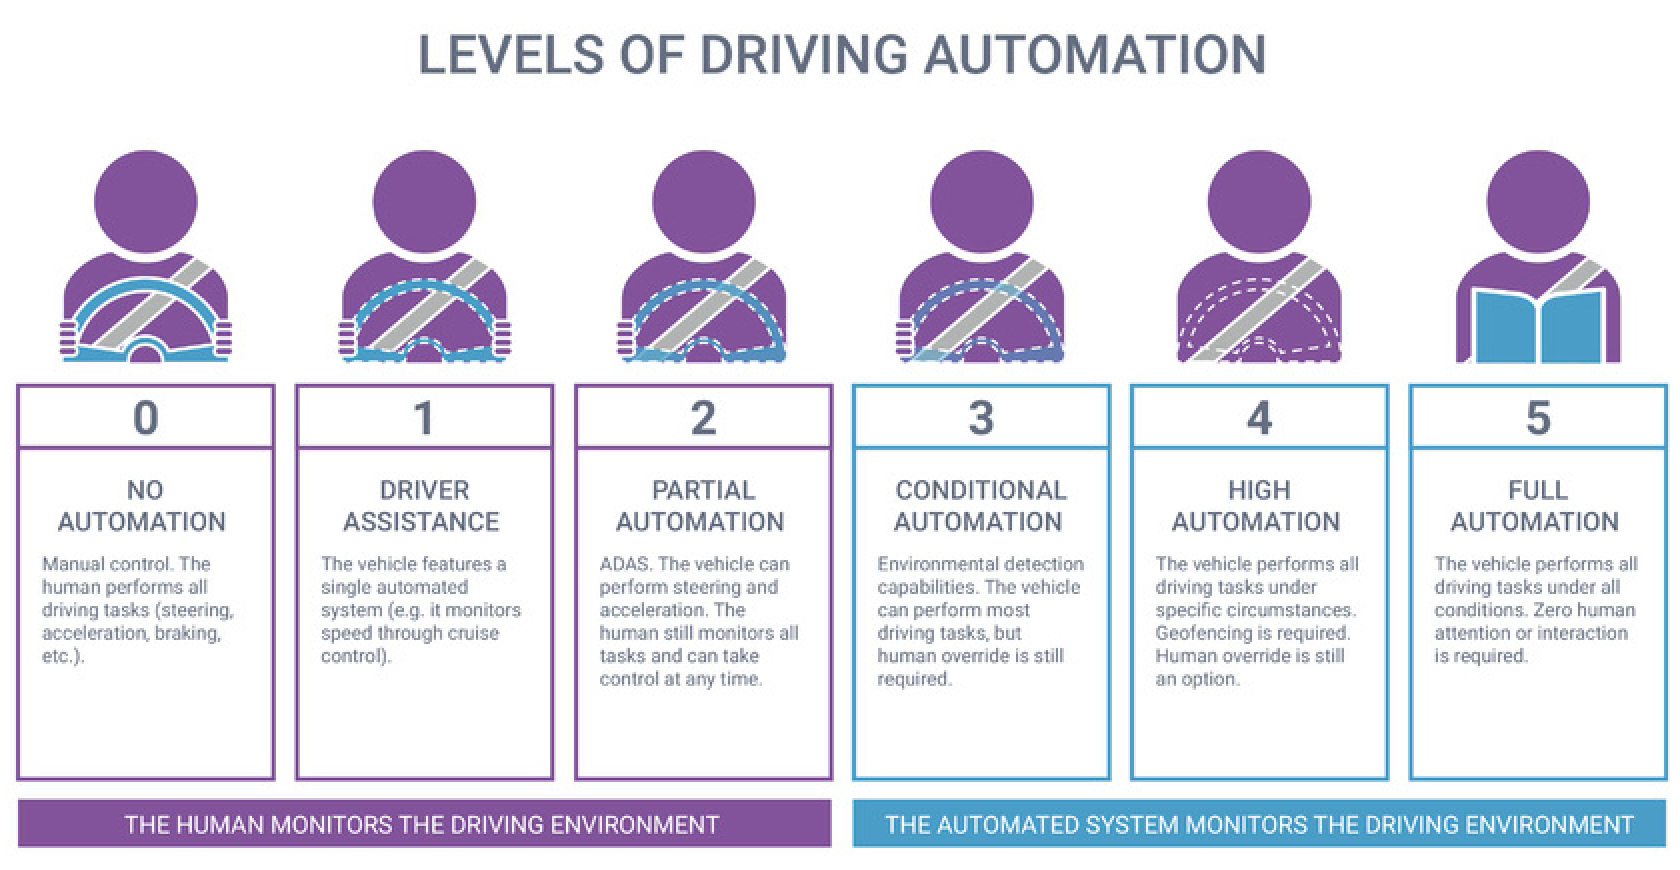
\includegraphics[width = 0.8\textwidth]{Images/six_levels_of_automation.png}
    \caption{Levels of automated driving}
    \label{fig:six_levels_of_autonomy}
\end{figure}

Moving on, it is relevant to mention that the classification of vehicles in terms of their autonomy is non-binary, meaning that there are not only fully autonomous vehicles and those entirely operated by humans, but various other levels of autonomy exist in between. This chapter will explain how autonomy levels are categorized and what level of autonomy is present in vehicles nowadays.

In 2014, The Society of Automotive Engineers (SAE) has proposed a standardization for categorizing the level of autonomy in vehicles, ranging from Level 0 (no automation) to level 5 (full automation) \cite{sae}. As shown in \autoref{fig:six_levels_of_autonomy}, these levels are determined by the extent to which the human and the automated system are involved in monitoring the environment and controlling the vehicle.

Currently, the majority of cars on the market fall into the lower levels of autonomy, with the driver still responsible for most aspects of driving. Some common automation features that new cars may offer to the owners include lane assisting, cruise control, automatic emergency braking, blind spot monitoring, automatic parking, autosteering and automatic lane changing.

Vehicles falling into the upper three categories are not yet available on the market, and it might be another several years until they become widely adopted. The main reasons for that are technological and regulatory challenges and public scepticism about AV safety.

Luckily, this article aims to address these questions by proposing a system for testing highly automated vehicles in a simulated environment, thus assessing whether the software agents controlling the vehicles are working as intended. More about that will be discussed in \autoref{chap:six}, when the proposed safety performance evaluation system is introduced.

\section{Safety of autonomous vehicles} \label{sect-2.4}
With regard to safety, there is a general belief that autonomous vehicles have the potential to improve transportation safety by addressing one of the leading causes of accidents and fatalities on the roads: human error. Drivers can be distracted by activities such as texting or talking on the phone or may become impaired or fatigued, leading to potentially dangerous situations. AVs, on the other hand, are equipped with sensors that constantly monitor their surroundings and detect potential hazards, allowing them to respond more quickly than a human driver could. This can be particularly important in emergencies, where reacting as quickly as possible might be vital.

Moreover, AVs can potentially eliminate road congestion and substantially improve traffic flow. Suppose there were no human-operated cars on the roads, and every participant would be operated by an AI with the ability to communicate among themselves and road infrastructure using radio waves. In that case, vehicles could better understand other vehicles' intentions and how the surrounding world will change. For instance, which driver might be turning soon, when the traffic light will change to green or where the road hazards are that should be avoided. If such communication were possible, travelling time would be reduced because all the vehicles would drive more efficiently.

In addition to improving overall road safety, AVs could help increase the mobility of people who cannot drive a car, for example, people with disabilities or older people.

However, it is essential to note that AVs also present potential risks, one being hardware malfunction and the other being cyber-attacks.
It is inevitable that mechanical components sometimes come with factory defects or develop a fault with time. They could contribute to inaccurate information that may lead to wrong and unsafe decision-making. For this reason, companies developing AVs must test all the critical components comprehensively to ensure their correctness. In addition, the future owners of the AVs must be provided with adequate systems that constantly check the state of the sensors and provide alerts that will announce the need for either technical service or recalibration if they are not in the optimal state.

Cyber-attacks could come into play anywhere where an AV communicates with online systems. It is inevitable that AVs, like other modern systems, will rely on external systems and services in one way or another. It could be by downloading software updates (which talking about the constantly evolving AV nature would be frequent), getting the latest traffic information for route planning, getting the weather forecast for traffic predictions or simply sending data to the manufacturer for analysis. All the information being sent can possibly be tampered with by malicious third parties and result in incorrect data, system faults and reduced safety.

Although it is crucial for AV manufacturers and regulators to prioritize safety in the design and operation of these vehicles, this research paper focuses solely on vehicle performance rather than correctness of their components and assumes that the systems are cryptographically safe and cannot be exploited by anyone. As mentioned in the book written by RAND Corporation in 2018 called “Measuring automated vehicle safety: Forging a framework”: Comparing these machines at vehicle (or higher) levels fits people’s intuition about safety \cite{fraade2018measuring}.